\PassOptionsToPackage{unicode=true}{hyperref} % options for packages loaded elsewhere
\PassOptionsToPackage{hyphens}{url}
%
\documentclass[ignorenonframetext,aspectratio=169]{beamer}
\usepackage{pgfpages}
\setbeamertemplate{caption}[numbered]
\setbeamertemplate{caption label separator}{: }
\setbeamercolor{caption name}{fg=normal text.fg}
\beamertemplatenavigationsymbolsempty
% Prevent slide breaks in the middle of a paragraph:
\widowpenalties 1 10000
\raggedbottom
\setbeamertemplate{part page}{
\centering
\begin{beamercolorbox}[sep=16pt,center]{part title}
  \usebeamerfont{part title}\insertpart\par
\end{beamercolorbox}
}
\setbeamertemplate{section page}{
\centering
\begin{beamercolorbox}[sep=12pt,center]{part title}
  \usebeamerfont{section title}\insertsection\par
\end{beamercolorbox}
}
\setbeamertemplate{subsection page}{
\centering
\begin{beamercolorbox}[sep=8pt,center]{part title}
  \usebeamerfont{subsection title}\insertsubsection\par
\end{beamercolorbox}
}
\AtBeginPart{
  \frame{\partpage}
}
\AtBeginSection{
  \ifbibliography
  \else
    \frame{\sectionpage}
  \fi
}
\AtBeginSubsection{
  \frame{\subsectionpage}
}
\usepackage{lmodern}
\usepackage{amssymb,amsmath}
\usepackage{ifxetex,ifluatex}
\usepackage{fixltx2e} % provides \textsubscript
\ifnum 0\ifxetex 1\fi\ifluatex 1\fi=0 % if pdftex
  \usepackage[T1]{fontenc}
  \usepackage[utf8]{inputenc}
  \usepackage{textcomp} % provides euro and other symbols
\else % if luatex or xelatex
  \usepackage{unicode-math}
  \defaultfontfeatures{Ligatures=TeX,Scale=MatchLowercase}
\fi
\usetheme[]{Frankfurt}
\usecolortheme{beaver}
% use upquote if available, for straight quotes in verbatim environments
\IfFileExists{upquote.sty}{\usepackage{upquote}}{}
% use microtype if available
\IfFileExists{microtype.sty}{%
\usepackage[]{microtype}
\UseMicrotypeSet[protrusion]{basicmath} % disable protrusion for tt fonts
}{}
\IfFileExists{parskip.sty}{%
\usepackage{parskip}
}{% else
\setlength{\parindent}{0pt}
\setlength{\parskip}{6pt plus 2pt minus 1pt}
}
\usepackage{hyperref}
\hypersetup{
            pdftitle={Genetic engineering in animals},
            pdfauthor={Deependra Dhakal},
            pdfborder={0 0 0},
            breaklinks=true}
\urlstyle{same}  % don't use monospace font for urls
\newif\ifbibliography
\setlength{\emergencystretch}{3em}  % prevent overfull lines
\providecommand{\tightlist}{%
  \setlength{\itemsep}{0pt}\setlength{\parskip}{0pt}}
\setcounter{secnumdepth}{0}

% set default figure placement to htbp
\makeatletter
\def\fps@figure{htbp}
\makeatother

% % set background image if you will
% \usebackgroundtemplate%
% {%
%     \includegraphics[width=\paperwidth,height=\paperheight]{02-dna_modification_background_dna_helix.jpg}%
% }

% % set caption font size
% % note that beamer presentation native captions have their own configs
% \usepackage{caption}
% \captionsetup{font=footnotesize}

% this font option is amenable for beamer
\setbeamerfont{caption}{size=\tiny}

% some beamer themes naturally might not support navigation symbols
% \setbeamertemplate{navigation symbols}{} % remove navigation symbols

\setbeamertemplate{footline}[page number] % insert page number in footline

% \setbeamertemplate{navigation symbols}{slide} % insert slide indication in navigation
% \setbeamertemplate{navigation symbols}{frame} % insert frame indication in navigation
% \setbeamertemplate{navigation symbols}{section} % insert section indication in navigation
% \setbeamertemplate{navigation symbols}{subsection} % insert subsection indication in navigation

% \AtBeginSubsection{} % supress subsection display

\title{Genetic engineering in animals}
\author{Deependra Dhakal}
\providecommand{\institute}[1]{}
\institute{GAASC, Baitadi \and Tribhuwan University}
\date{Academic year 2019-2020}

\begin{document}
\frame{\titlepage}

\begin{frame}
\tableofcontents[hideallsubsections]
\end{frame}
\hypertarget{transgenic-animals}{%
\section{Transgenic animals}\label{transgenic-animals}}

\begin{frame}{Background}
\protect\hypertarget{background}{}

\begin{itemize}
\tightlist
\item
  Woollier sheep and smarter sheep dogs have both been improved through
  many generations of selective breeding
\item
  Obviously, the more we know about genetics, the faster and more
  effectively we can improve our crops and livestock
\item
  Most early experiments in animal transgenics were done with mice
\item
  Now engineered animals:

  \begin{itemize}
  \tightlist
  \item
    Sheep, goats, cats, dogs and monkeys
  \end{itemize}
\item
  Transgene may be derived from same or from distantly related animals,
  or even from unrelated organisms.
\end{itemize}

\end{frame}

\begin{frame}{Creating transgenic animals: Nuclear microinjection}
\protect\hypertarget{creating-transgenic-animals-nuclear-microinjection}{}

\begin{figure}
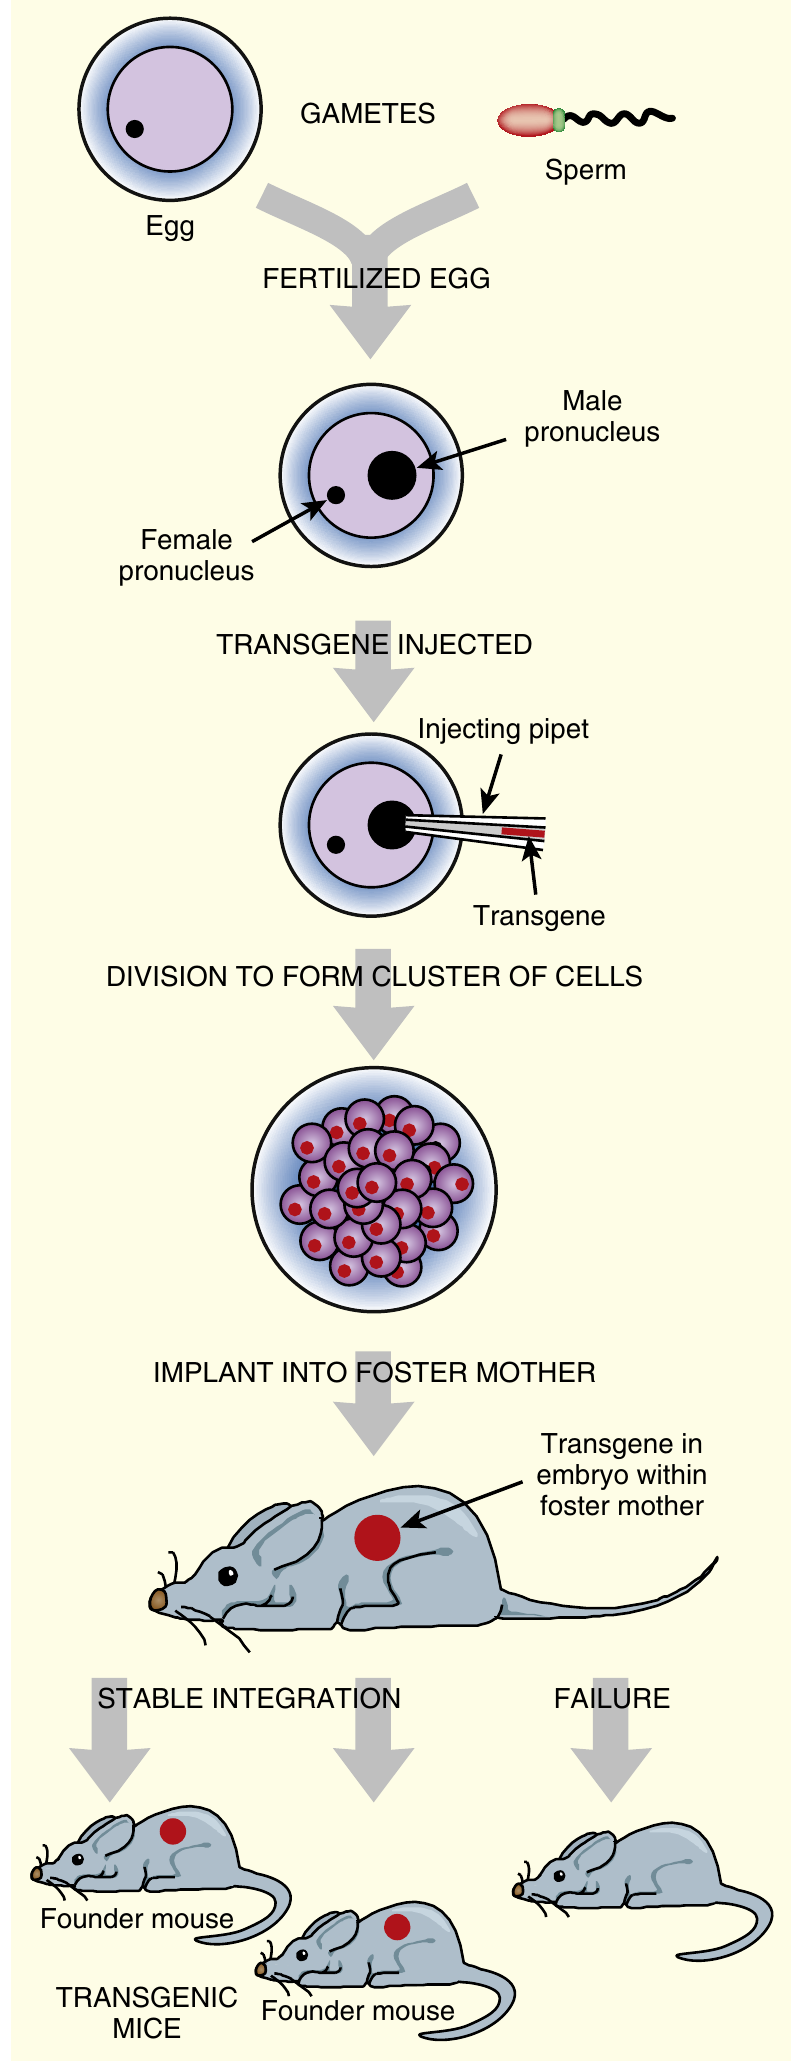
\includegraphics[width=0.16\linewidth]{../images/transgenic_mice} \caption{\textbf{Creation of Transgenic Animals by Nuclear Injection}\newline In vitro fertilization is used to start a transgenic animal. Harvested eggs and sperm are fertilized, and before the pronuclei fuse, the transgene is injected into the male pronucleus. The embryo continues to divide in culture and is then implanted into a mouse. The “foster mother” mouse has been treated with hormones so that she accepts the embryo and carries on with the pregnancy. The offspring are screened for stable integration of the transgene. Founder mice have one copy of the transgene.}\label{fig:transgenic-animals}
\end{figure}

\end{frame}

\begin{frame}{Creating transgenic animals: Nuclear microinjection}
\protect\hypertarget{creating-transgenic-animals-nuclear-microinjection-1}{}

\begin{itemize}
\tightlist
\item
  Transgene is injected into fertilized egg cells
\item
  Soon after fertilization, individual nuclei from both sexes are
  separate as pronuclei.
\item
  Before pronuclei fuse together, DNA is injected into male pronucleus.
\item
  Success rate: 5\% - 40\%
\item
  After culturing for few days \emph{in-vitro}, embryo is then implanted
  into womb of a female animal -- the \textbf{foster mother}.
\item
  Those that received the transgene and maintain it stably are called
  founder animals.
\end{itemize}

\end{frame}

\begin{frame}{Comparison of recombinant protein expression systems}
\protect\hypertarget{comparison-of-recombinant-protein-expression-systems}{}

\begin{figure}
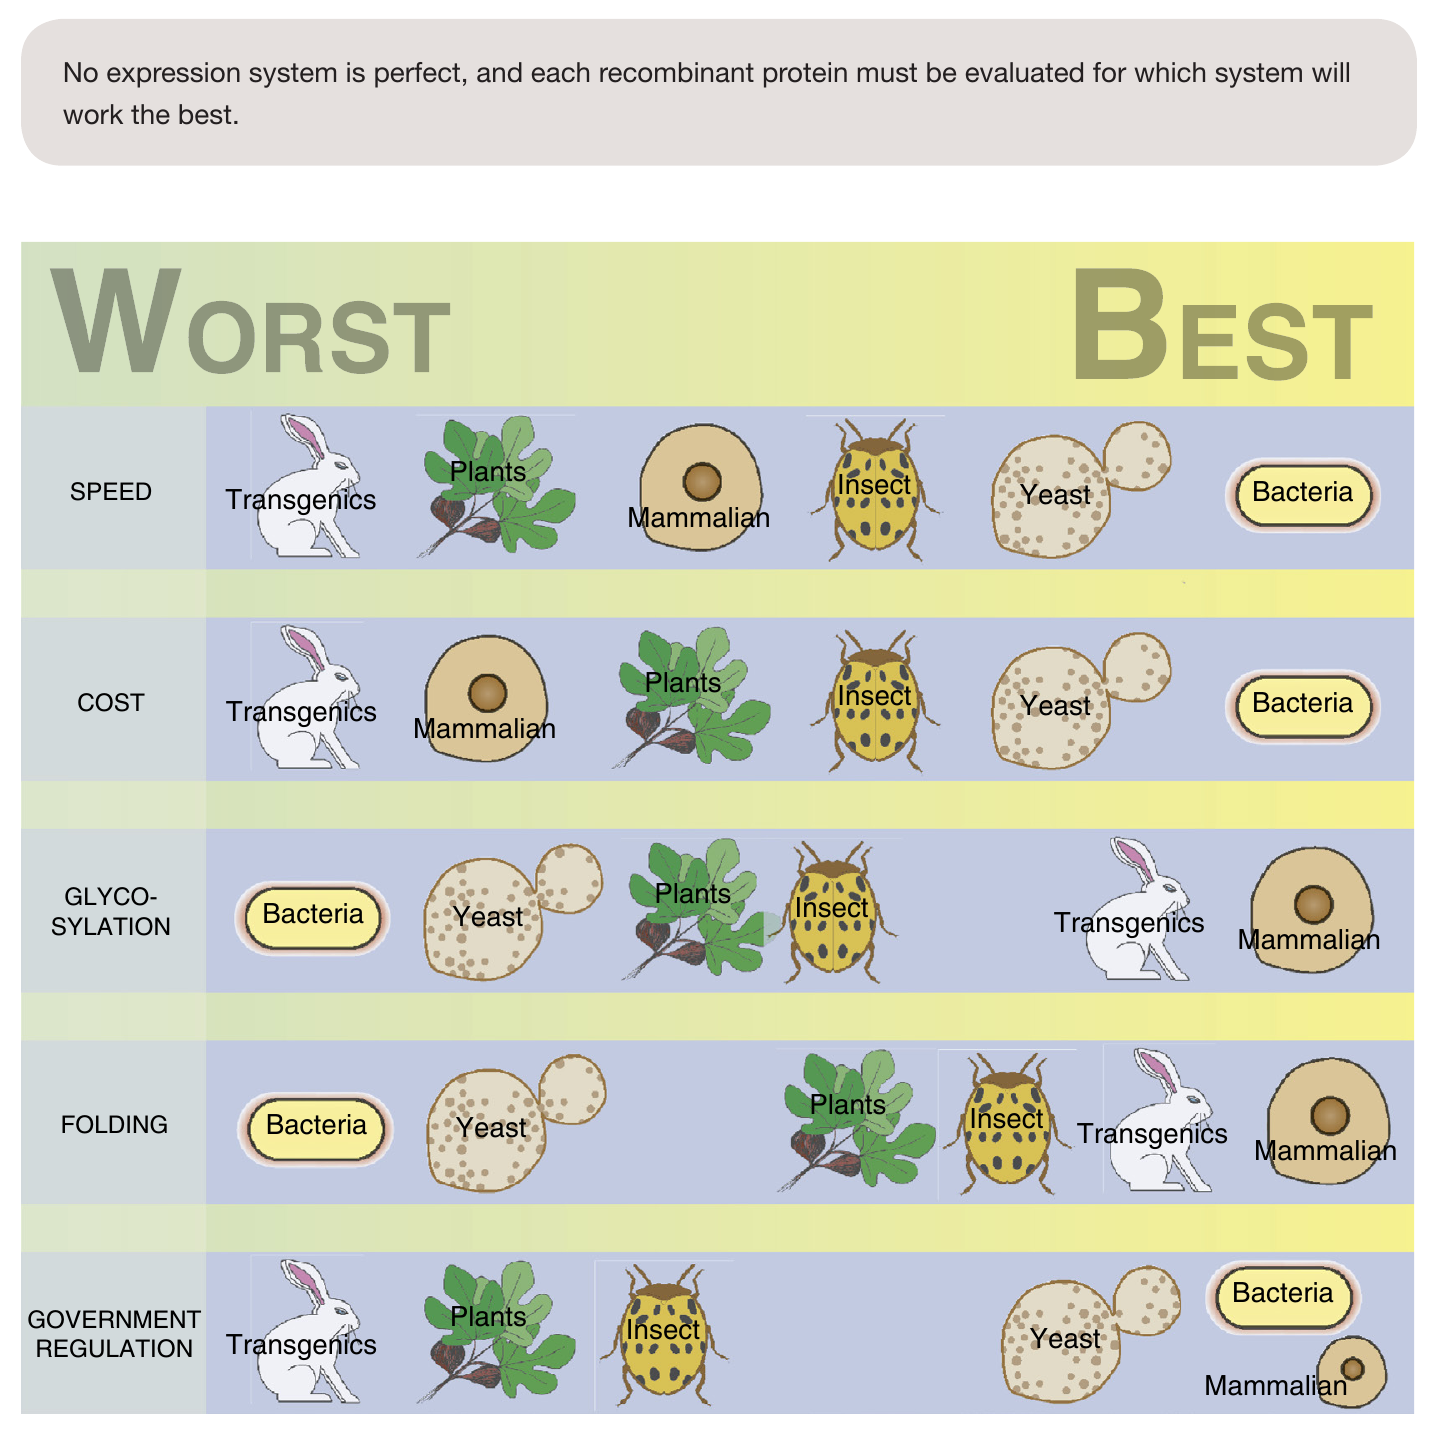
\includegraphics[width=0.4\linewidth]{../images/system_comparison} \caption{Each protein expression system falls on a continuum of worst to best for characteristics such as speed, cost, glycosylation, folding, and government regulations. The other symbols include cultured mammalian cells, insect cells, yeast, and bacteria.}\label{fig:system-comparision}
\end{figure}

\end{frame}

\begin{frame}{Comparison of recombinant protein expression systesm:
Insects}
\protect\hypertarget{comparison-of-recombinant-protein-expression-systesm-insects}{}

\begin{figure}
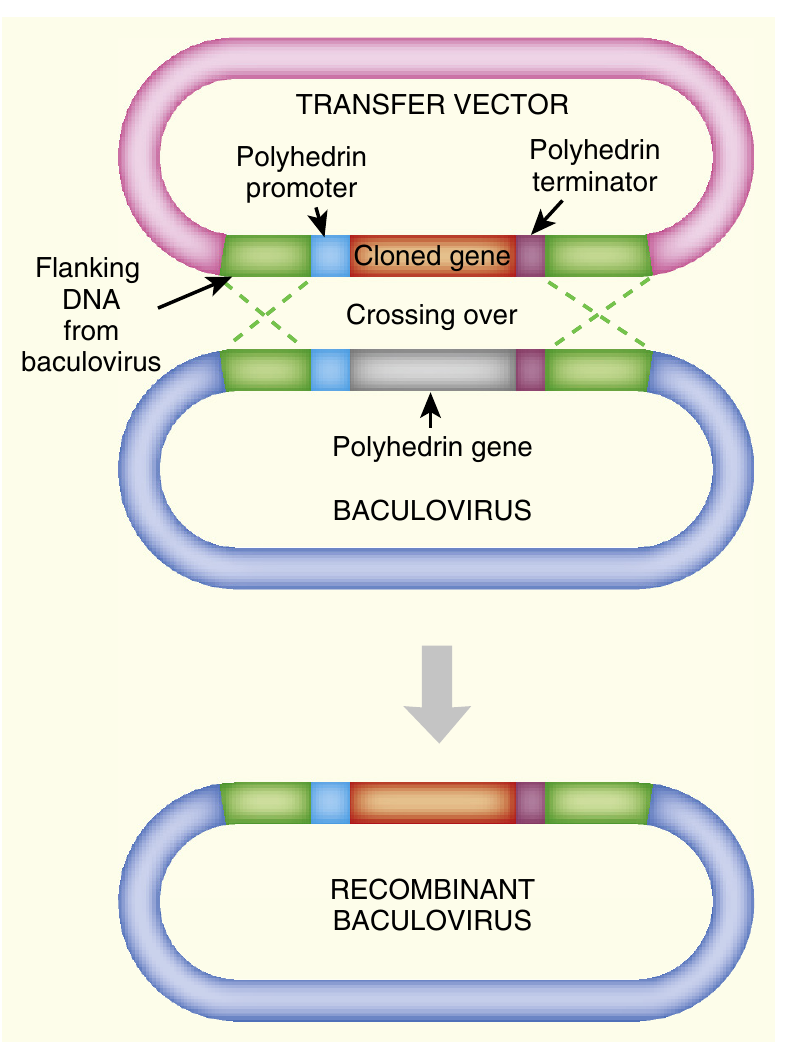
\includegraphics[width=0.3\linewidth]{../images/baculovirus_expression_vector} \caption{\textbf{Baculovirus Expression Vector} \newline To express a gene in insect cells, the gene must be inserted into a baculovirus genome. First, the gene of interest is cloned into a transfer vector containing the baculovirus polyhedrin gene promoter followed by a multiple cloning site and the polyhedrin terminator. This is done in E. coli. The construct is transfected into insect cells along with the normal baculovirus genome. A double crossover between the polyhedrin promoter and terminator replaces the polyhedrin gene with the gene of interest.}\label{fig:baculovirus-insect}
\end{figure}

\end{frame}

\begin{frame}{Comparison of recombinant protein expression systesm:
Insects}
\protect\hypertarget{comparison-of-recombinant-protein-expression-systesm-insects-1}{}

\begin{itemize}
\tightlist
\item
  One of most often used is multiple nuclear polyhedrosis virus (MNPV).
\item
  It infects many insects and replicates well in many cultured insect
  cell lines. A popular cell line used to propagate this baculovirus is
  from the fall armyworm ( \emph{Spodoptera frugiperda}).
\end{itemize}

\end{frame}

\begin{frame}{Control of expression}
\protect\hypertarget{control-of-expression}{}

\begin{itemize}
\tightlist
\item
  Transgenes may be artificially regulated by a variety of control
  systems.
\item
  Engineered versions of the bacterial lac and tet regulators are widely
  used.
\item
  Transgene expression may be controlled by site-specific recombination.
  Either the Cre or Flp recombinase can rearrange segments of transgenic
  DNA to turn transgenes on or off.
\item
  A similar approach uses bacterial recombinases, such as the \(\Phi\)
  C31 integrase.
\end{itemize}

\end{frame}

\begin{frame}{Applications}
\protect\hypertarget{applications}{}

Marathon Mouse can run about 1800 meters -- more than a mile -- before
exhaustion. This is twice as far as a normal mouse can last. Marathon
mouse has enhanced PPAR-delta-a regulator of several genes involved in
burning fat and in muscle development.

Mighty Mouse was engineered to lack myostatin, a protein that slows
muscle growth. The result is colossal muscle development. There is one
known case of a human with a genetic defect leading to lack of
myostatin. A German boy, born in Berlin in 2000, has muscles twice the
size of other children his age.

\end{frame}

\begin{frame}{Applications}
\protect\hypertarget{applications-1}{}

\begin{figure}
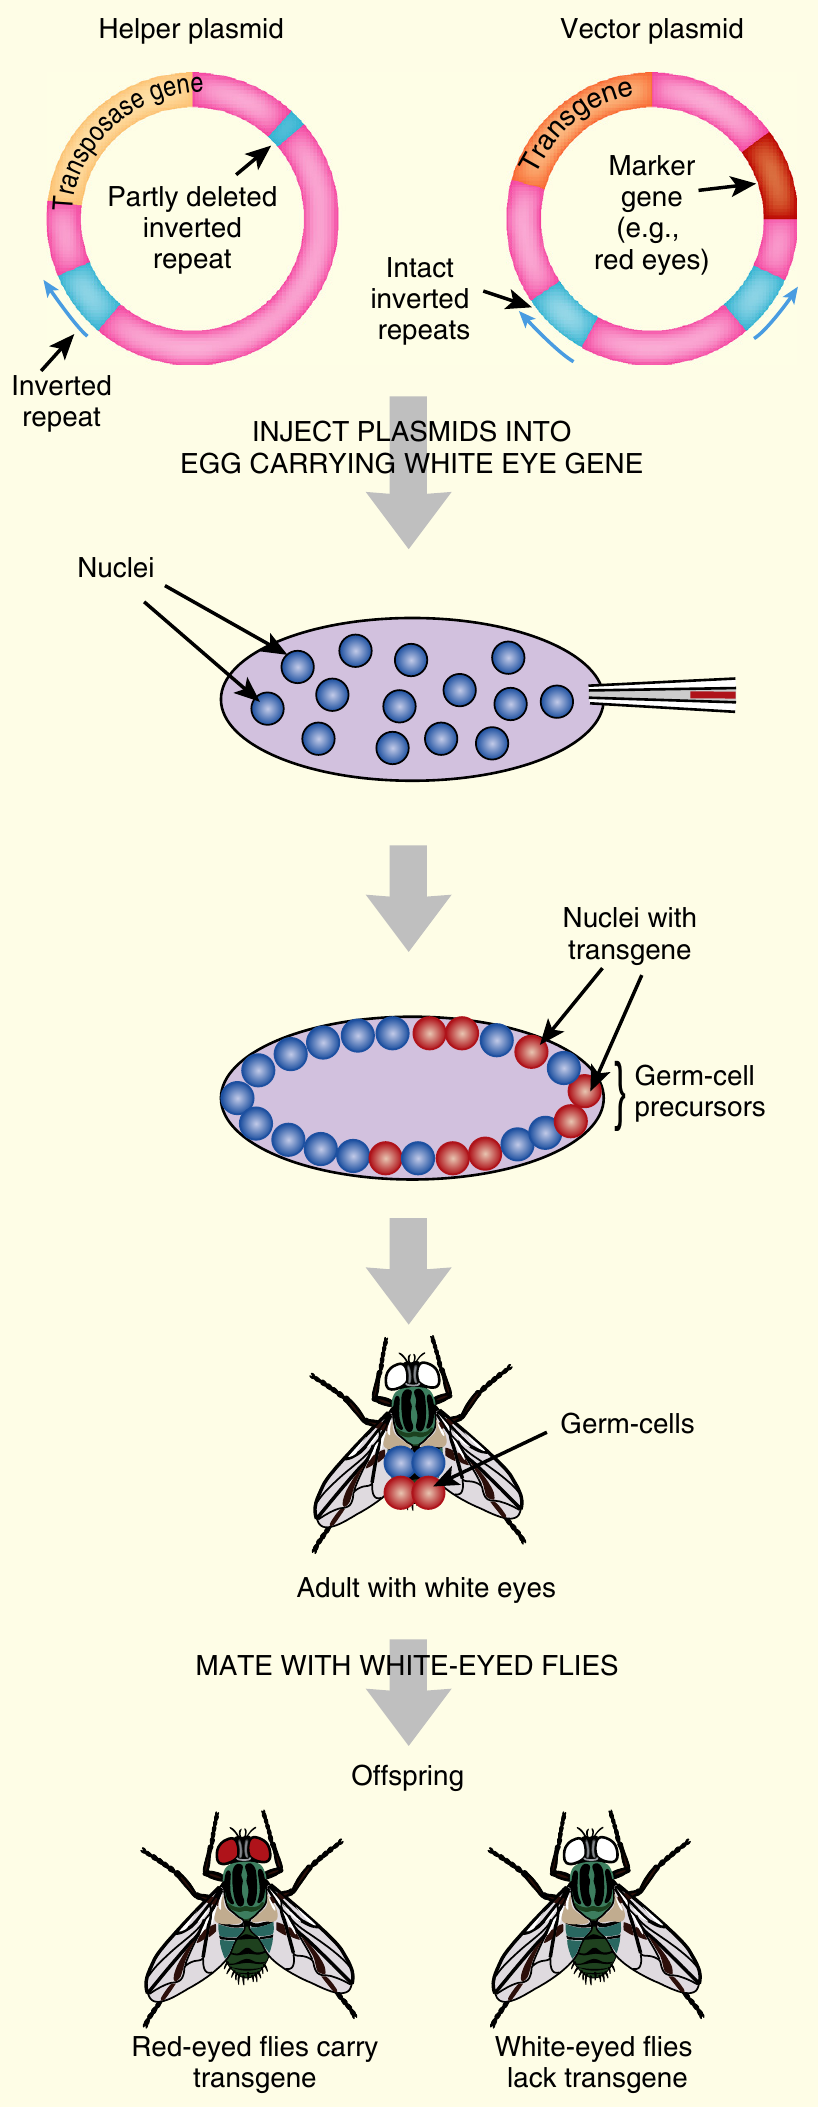
\includegraphics[width=0.2\linewidth]{../images/transgenic_insects} \caption{\textbf{Element engineering in Drosophila} \newline Two different plasmids are used to insert transgenes into Drosophila. The helper supplies the transposase. It carries an immobile P element with one of the inverted repeats deleted but with functional transposase. The second plasmid has the transgene plus marker (a gene for red eyes) flanked by the P element inverted repeats. Both vectors are injected into the posterior end of an egg, which has 2000 to 4000 nuclei within one membrane. The transposase is expressed, which results in random transposition of the transgene (plus marker) into various chromosomes in different nuclei. Hopefully, some insertions occur in germ cell nuclei. The egg is then allowed to form an adult (with white eyes in this case). This fly is then mated to another white-eyed adult. If insertion into the germline was successful, some offspring will express the marker gene and have red eyes.}\label{fig:insect-transgenics}
\end{figure}

\end{frame}

\begin{frame}{Applications: other}
\protect\hypertarget{applications-other}{}

\begin{itemize}
\tightlist
\item
  Transgenic animals help fight diseases (Lysozyme fortified livestock
  milk to prevent diarrhoeal disease)
\item
  Genetically modified mosquitoes
\item
  Growth promoter genes in Atlantic salmon
\end{itemize}

\end{frame}

\end{document}
